%\stepcounter{contsubsec} 
\section{INTRODUCCIÓN}

La determinación y el control de actitud en satélites son esenciales para el éxito de una misión espacial. Existen diferentes métodos de control de actitud, los cuales pueden clasificarse como pasivos y activos. El control pasivo recurre principalmente al diseño geométrico y magnético del satélite, buscando aprovechar los principios físicos y fuerzas naturales que actúan sobre el satélite, aumentando los efectos de una mientras se minimizan los de otras. Por otro lado, el control activo emplea actuadores como propulsores, magnetorquers (barra de torsión) o ruedas de reacción (Reaction Wheels, RW)  para modificar la actitud del satélite mediante la generación de torques correctivos [1]. Durante una misión espacial, se pueden utilizar diferentes modos de control de actitud para sus diferentes fases y tareas del satélite.
En los últimos años, se ha presentado un aumento de misiones espaciales que involucran CubeSats, el cual es un tipo de nanosatélite formado a partir de unidades cúbicas (U) de 10 cm de lado, y que cada vez presentan una mayor complejidad. Por lo tanto, ha sido de gran interés el incremento de la vida útil y el rendimiento de las misiones, donde el sistema de determinación y control de actitud (Attitude Determination and Control System, ADCS)  juegan un papel fundamental para garantizar la probabilidad de éxito [2]. En este sentido, el control de actitud de un CubeSat es fundamental para cumplir el perfil de misión, normalmente situado en órbita baja (Low Earth Orbit, LEO),  donde se busca tener precisión de apuntamiento y estabilidad para las cargas útiles, antenas y paneles solares, que son componentes críticos para el funcionamiento de la nave espacial y del éxito de la misión.
El control de actitud en CubeSats es normalmente provisto por RW, las cuales intercambian momento con la nave sin consumir propelente. No obstante, una desventaja de este tipo de dispositivos electromecánicos es que acumulan el momento para mantener una actitud deseada y, en consecuencia, las RW se saturan cuando alcanzan su velocidad máxima de rotación lo cual impiden que estas puedan intercambiar momentos que garanticen a la estabilidad del satélite. Por tal motivo, surge un desafío en el área de control de actitud que busca la desaturación de dichas ruedas de reacción mientras se conserva la actitud del satélite.
Algunos de los desafíos que se presentan frente a este fenómeno se deben a que comúnmente el control de actitud y la desaturación de RW son tratados por separado, y a pesar de que existen numerosos estudios sobre el control de actitud con torques magnéticos, hay pocos artículos que involucran la desaturación del momento de las RW mediante magnetorques [3]. Por otro lado, se requieren controladores que garanticen la estabilidad del satélite anticipando y actuando ante perturbaciones presentes en el ambiente espacial como por ejemplo torques externos debido a gradientes gravitacionales, torques aerodinámicos o torques de radiación solar [4].
Debido a esto, es de particular interés estudiar técnicas de desaturación con controladores, que permitan asistir estos dispositivos recurriendo a otros actuadores auxiliares como los magnetorques, los cuales, por medio de su interacción con campos magnéticos, generan un par que desatura las ruedas de reacción. No obstante, a diferencia de las RW que pueden generar un torque en cualquier dirección y en cualquier momento, los magnetorques dependen de la interacción con el plano ortogonal del campo geomagnético instantáneo, el cual cambia a medida que el satélite orbita alrededor de la tierra [5]. Adicionalmente, a pesar de que los magnetorques son dispositivos confiables en LEO, producen una respuesta más lenta en comparación con otros actuadores lo cual reduce la capacidad de maniobra del satélite y su tiempo de reacción ante perturbaciones externas.
En este sentido, se propone evaluar estrategias de control de actitud que incorporen la desaturación de las ruedas reacción, mediante simulaciones computacionales a partir de un modelo dinámico basado en el CubeSat de entrenamiento EyasSat [6]. Adicionalmente, se pretende realizar una comparación de diferentes controladores bajo algunos escenarios o perfiles de misión propuestos, con el fin de determinar las condiciones donde mejor se desempeñan las estrategias de control propuestas. La elección de este modelo en particular de CubeSat se debe a que dicho satélite se encuentra disponible en el programa de Ingeniería Aeroespacial; y es de especial interés incluirlo en el planteamiento de las simulaciones porque puede ser aprovechado junto con otros equipos, como la Jaula de Helmholtz, para consolidar una futura línea de investigación en control satelital.


\newpage
%--------------------------------------------

%Las \section{} que para esta plantilla son los títulos de nivel 1 siempre inician en una página nueva. Las \subsection{} y demas particiones de niveles 2 al 4 pueden ir en medio de una página.

\section{PLANTEAMIENTO DEL PROBLEMA}

Se refiere al interrogante que lleva al investigador a buscar respuestas concretas. Es la definición del problema que aborda con la investigación. 

\subsection{Antecedentes}

Los antecedentes son las investigaciones que se han realizado previamente y que guardan una relación histórica con el tema de investigación actual. 

\newpage
%-------------------------------


\section{JUSTIFICACIÓN}

Responde a los interrogantes del por qué se desea conocer el tema y por qué se seleccionó, así como cuál es el aporte que tendrá el texto a la ciencia. 

No abuse del uso de \textit{cursivas} o \textbf{negritas} dentro del texto, úselas muy moderadamente, por lo general saturan y dificultan la lectura del documento. Utilice cursivas en casos muy particulares como géneros y especies (\textit{Tyrannus melancholicus}), términos químicos (\textit{kr}), letras griegas ($\beta$) y algunos títulos y subtítulos. El entorno matemático de \LaTeX \ muestra las variables y símbolos en letra cursiva, asegurese de hacer lo mismo al referenciarla en el documento, Utilice \textbf{negritas} en algunos títulos de capítulos y subcapítulos, algunos datos de tablas o enfatizar aspectos muy particulares. El uso de \underline{texto subrayado} no se recomienda en normas IEEE.

Utilice moderadamente el uso de abreviaturas, se prefiere que el texto sea más largo y claro que corto y confuso para el lector. Por ejemplo, IEEE puede significar Institute of Electrical and Electronics Engineers o Instituto Español de Estudios Estratégicos. Sin embargo, las abreviaturas pueden ser útiles en casos como la repetición continua en un mismo párrafo.

Prefiera las comillas “inglesas” y ‘sencillas’ por sobre las «latinas» o «españolas».

\begin{description}
    \item[Características:] texto descriptivo.
    \item[Propiedades:] texto descriptivo.
    \item[Estructura:] texto descriptivo.
\end{description}

\newpage
%--------------------------
\section{OBJETIVOS}

\subsection{Objetivo general}

El objetivo general y los objetivos específicos describen lo que se pretende con la investigación, cuál es el alcance y cuál es el problema que se desea resolver. Deben iniciarse con verbos que describan claramente lo que se lleva a cabo.

\subsection{Objetivos específicos}

Se describen algunos ejemplos de verbos comunes que se utilizan en el planteamiento de objetivos, los cuales cambiarán dependiendo de su investigación.

\begin{itemize}
    \item Describir.
    \item Analizar.
    \item Demostrar.
    \item Probar.
    \item Comparar.
    \item Definir.
    \item Establecer.
    \item Interpretar.
\end{itemize}

\newpage
%--------------------------
\section{PROBLEMA DE INVESTIGACIÓN}

El problema de investigación es el enunciado de lo que puede ser demostrado o encontrado, y de lo cual se requieren pruebas y evidencias.

\newpage
%--------------------------
\section{HIPÓTESIS}

La hipótesis es la creencia, la suposición o la conjetura de un fenómeno posible, es decir, independiente de si es verdadero o no. En la hipótesis se reúnen datos, se comparan y se escogen las explicaciones más probables. Dicho de otra forma, la hipótesis es la explicación probable de la relación entre dos o más variables.

    \subsection{Hipótesis de trabajo}

    Texto descriptivo.

    \subsection{Hipótesis estadística}

    Texto descriptivo.
    
        \subsubsection{Hipótesis nula:}
texto descriptivo inicia en la misma línea y continúa como párrafo normal IEEE.

        \paragraph{Hipótesis alternativa:}
texto descriptivo inicia en la misma línea y continúa como párrafo normal IEEE.
        

\newpage
%--------------------------
\section{MARCO TEÓRICO}

En esta sección se citan los autores que han tenido influencia directa en tu investigación. Recuerda, debes escoger solo un método para realizar las citas y referencias, es decir, debes seleccionar entre gestores especializados como Mendeley, Zotero, EndNote, etc., Microsoft Word, o “Manuales”; no se deben mezclar entre sí. Nuestra recomendación principal es Mendeley. Evita referenciar sitios como blogs, Wikipedia, Rincón del Vago, Monografías.com y demás portales web que no se consideran fuentes primarias. No limites tu búsqueda a una sola herramienta (por ejemplo, solo www.google.com). Realiza búsquedas en diferentes plataformas académicas, tales como:

\begin{itemize}
    \item \textbf{Catálogo Sistema de Bibliotecas UdeA:} material impreso que reposa en Bibliotecas UdeA, tales como libros, revistas, tesis, diccionarios, informes, etc.
    \item\textbf{Bases de datos suscritas de la Biblioteca:} plataformas digitales con millones de documentos en texto completo.
    \item\textbf{Bases de datos de libre acceso:} Google Scholar, Microsoft Academic, Google Books, Redalyc, Scielo, Dialnet, DOAJ, PubMed, Base Search, entre muchas más.
    \item\textbf{Documentos con acceso restringido:} si requieres el texto completo de artículos o libros con acceso restringido, que por lo general se encuentran en bases de datos no suscritas por la Universidad de Antioquia, solicítalos en tu Biblioteca enviando título exacto, el DOI o la url del documento. Tenemos convenios nacionales e internacionales que nos permiten acceder a esta información.
\end{itemize}

Ejemplo de cita parafraseada, es decir, frase no textual adaptada con las palabras de quien escribe; esta forma de citación es la más adecuada en textos académicos, demuestran lectura, análisis y redacción propia \cite{sec:pediatria}. Ejemplo de “Cita textual menor a 40 palabras, al interior del párrafo; no utilice recurrentemente esta forma de citación, pues demuestra poco análisis y redacción propios” \cite[p. 9]{opc:ramirez}. Otros ejemplos aceptados en estilo IEEE 2020:

En citas paráfrasis, es posible mencionar o no el o los autores en la oración, ejemplos: resultados demostrados por Arango \cite{sec:pediatria}, resultados demostrados mediante publicación científica \cite{sec:pediatria}. Cita en paráfrasis de dos autores, con o sin autor mencionado: datos suministrados por Ramírez y Guzmán \cite{opc:ramirez}, datos suministrados en revista académica \cite{opc:ramirez}. Cita en paráfrasis con tres o más autores con et al.: resultados publicados por Baker et al. \cite{art:baker}, resultados publicados en revista científica \cite{art:baker}. Cita con dos fuentes, cada una en corchetes y en orden numérico: ambos autores coinciden en estos datos \cite{opc:bbva}, \cite{opc:film}. Cita con tres fuentes o más, con corchetes para el primero y el último, en orden numérico y separados por guion: diversos autores coinciden en estos datos \cite{opc:bbva}–\cite{lib:ieee}. 

Cita “textual menor a 40 palabras” \cite[p. 466]{art:espectador}, cita “textual menor a 40 palabras con páginas continuas o discontinuas” \cite[pp. 15-16]{tes:tesis}.  %[8, pp. 15-16). debe terminar en parentesis

Cita de cita en paráfrasis mencionando o no autores: Quintero y González, citados por Rioja \cite{con:conferencia}, Quintero y González, citados por \cite{con:conferencia}. Cita textual mayor a 40 palabras sin comillas:


    \begin{quotation}
    Es importante destacar que la revisión realizada permitió definir el constructo a evaluar, es decir, especificar el concepto de la e-inclusión que se asume en la investigación, así como los factores que deben ser considerados para su evaluación. Lo anterior constituye el fundamento conceptual de la tesis y es la base para desarrollarla \cite[p. 107]{art:acimed}. 
    \end{quotation}

Cita textual o directa con más de 40 palabras (se omiten las comillas), bloque aparte, sangría 1.25 cms. Ya que IEEE no señala nada en particular de este caso, se adaptan de las normas APA. Datos estadísticos analizados con SPSS \cite{opc:ibm}. Procure no incurrir en la citación excesiva: 

\newpage
%--------------------------
\subsection*{MÉTODO PARA ELABORAR CITAS Y REFERENCIAS}

Recuerda, debes escoger solo un método para realizar las citas y las referencias, es decir, debes seleccionar entre un gestor especializado como Mendeley, Zotero o EndNote (confiabilidad alta), el gestor nativo Microsoft Word (confiabilidad media) o “manuales” (confiabilidad baja); no se deben mezclar entre sí, nuestra recomendación principal es Mendeley, pues te permite almacenar, subrayar e insertar notas en PDF´s, guardar fichas bibliográficas, elaborar citas y bibliografías en APA, Vancouver, IEEE y más de 1.000 estilos diferentes, exportar registros, compartir documentos, etc. Para mayor información de Mendeley.com y \LaTeX visitar:

\url{http://tiny.cc/zzrnuz}

La presente plantilla incluye los archivos requeridos para la construcción apropiada de las referencias bibliograficas bajo los parametros de las normas IEEE, todo se limita a modificar los campos del archivo \textit{refe.bib} segun las necesidades de su escrito. Aqui algunos ejemplos de los diferentes tipos de documentos referanciables.


Refencia a un libro \cite{lib:libro}, a un artículo \cite{art:baker}, a una seccion de libro sin título \cite{sec:pediatria}, a un acta \cite{act:acta}, a una conferencia \citep{con:conferencia}, a un capítulo o páginas específicas con título propio de un libro\citep[pp. 7-10]{ent:entre_libro},  a un documento sin editorial \citep{fll:folleto}, a las memorias de una conferencia \citep{ina:articulo_en_acta}, a un informe técnico \citep{inf:informe_tecnico}, a un manual \citep{man:manual}, a una tesis doctoral \citep{phd:phd_tesis}, a una tesis de maestría \citep{tes:tesis}, a una web o información de internet \citep{web:web} y para otros tipos de referencias diferentes a las anteriores \cite{opc:film}. Para el listado de referencias, tenga en cuenta que el apellido principal será la última palabra en el campo \textit{author}; Si como autor no figura una persona sino una organización, al llenar el campo \textit{author} del archivo \textit{.bib}, use $\{\}$ dobles (ver referencia \citep{lib:ieee}).

A continuación se muestra una de las referencias del archivo \textit{refe.bib}, donde \linebreak \textit{ent:entre\_libro} es el identificador de la misma y para referenciarla se debe escrbir el comando $\backslash cite\{ent:entre\_libro\}$ 

\newpage
\begin{verbatim}
@inbook{ent:entre_libro,
     author         = {Angela Zapata},
     title          = {Titulo de libro},
     chapter        = {},
     pages          = {10-20},
     publisher      = {Editor},
     volume         = {},
     series	        = {},
     type           = {},
     address        = {},
     edition        = {},
     year           = {20XX},
     month          = {},
     note           = {},
     language       = {},
     }
\end{verbatim}

Recuerde que \LaTeX , en la sección de referencias, solo muestra las que se han citado en su escrito; agregar la información en el archivo \textit{refe.bib} no implica que la referencia se muestre en su documento

Por otro lado, para citar ecuaciones e información semejante dentro del texto use $\backslash ref\{\}$, por ejemplo (\ref{eq:maxwell}) o (\ref{eq:maxwell3})

\begin{equation}\label{eq:maxwell}
    \oint_C \vec{B}\cdot d \vec{l}=\mu_0\int_S \vec{J}\cdot d \vec{s}+\mu_0\epsilon_0\dfrac{d }{d t}\int_S \vec{E}\cdot d \vec{s}
\end{equation}

y a su vez

\begin{gather}
    \vec{\nabla}\cdot \vec{E}= \dfrac{\rho}{\epsilon_0}\\
    \vec{\nabla}\cdot \vec{B}= 0\\
    \vec{\nabla}\times\vec{E}=-\dfrac{\partial\vec{B}}{\partial t}\\
    c^2\vec{\nabla}\times\vec{B} =\dfrac{\vec{J}}{\epsilon_0}+\dfrac{\partial
\vec{E}}{\partial t}\label{eq:maxwell3}\\
    \vec{\nabla}\times \vec{B}=\mu_0\vec{J}+\mu_0 \epsilon_0 \dfrac{\partial \vec{E}}{\partial t}
\end{gather}


\newpage
%--------------------------
\section{METODOLOGÍA}

En la metodología se establecen los enfoques de investigación, esto es, cuantitativo, cualitativo o mixto.

\newpage
%--------------------------
\section{RESULTADOS}

En los resultados se comunican los hallazgos y descubrimientos del estudio. Se incluyen tablas, figuras, diagramas y demás material demostrativo.




 Al narrar descriptivamente una figura, tabla, etc., en un párrafo, puedes insertar una referencia cruzada, es decir, un hipervínculo al elemento mencionado dentro o fuera de paréntesis, ejemplos: estos resultados se muestran en la \textbf{Tabla \ref{table:prob_milenio}}.  Igualmente, los datos son validados con otros instrumentos \textbf{(Tabla \ref{table:num_mersenne}, Tabla \ref{table:medalla_fields})}. Lineamientos que se establecen en la nueva versión de las Normas APA séptima edición \textbf{(Fig. \ref{figportada_apa})}. La producción intelectual institucional se publica en el Repositorio \textbf{(Fig. \ref{fig:escudo_udea})}. Si la figura es de tu completa autoría, \textbf{NO} es necesario colocar la leyenda “Elaboración propia” \textbf{(Fig. \ref{fig:hiperbolica})}.

\begin{figure}[!ht]
    \begin{center}
    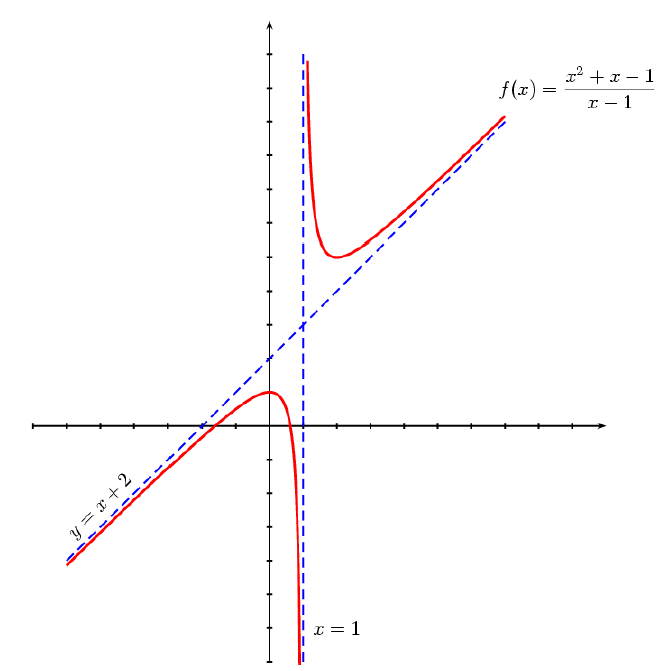
\includegraphics[scale=0.5]{imagenes/grafica.png}\\
    \end{center}
    \caption{Función hiperbólica}
    \label{fig:hiperbolica}
    \textit{}
\end{figure}

\begin{table}%[!ht]
\caption{\MakeUppercase{Problemas del milenio: la resolucion de uno de estos problemas se premian con un monto de us\$ 1 millon}}
\begin{center}
\begin{tabular}{  l c }
    \hline
    1 & El problema de $P$ frente a $NP$  \\ \hline
    2 &  La conjetura de Hodge \\ \hline
    3 &  La conjetura de Poincaré \\ \hline
    4 &  La hipótesis de Riemann \\ \hline
    5 &  Yang-Mills y el salto de masa ("mass gap")\\ \hline
    6 &  Las ecuaciones de Navier-Stokes\\ \hline
    7 &  Conjetura de Birch y Swinnerton-Dyer\\
        \hline
\end{tabular}
\end{center}
\label{table:prob_milenio}
\end{table}

%\clearpage

\begin{table}%[!ht]
\caption{\MakeUppercase{Medalla Fields: matemáticos galardonados con este premio desde 2010; la medalla Fields se comenzó a entregar desde 1936}}
\begin{center}
\begin{tabular}{cp{4cm}p{2.5cm}p{6cm}}
    \hline
    año & Ganador(es) & pais & universidad/instituto\\
    \hline 
        2010 & Elon Lindenstrauss & Israel & Universidad Hebrea de Jerusalén\\
         & Ngo Bao Chau ,  & Vietnam y Francia &Paris-Sud 11 University y Institute for Advanced Study \\
         & Stanislav Smirnov  & Rusia & Universidad de Ginebra\\
         & Cédric Villani & Francia & Institut Henri Poincaré\\
         \hline
         2014 & Artur Ávila  & Francia &Instituto Nacional de Matemática Pura y Aplicada \\
         & Manjul Bhargava  &  Canadá y Estados Unidos &Universidad de Princeton \\
         & Martin Hairer & Austria & Imperial College London\\
         & Maryam Mirzajani & Irán &Universidad Stanford \\
         \hline\\
         2018	 & Caucher Birkar & Irán y Reino Unido & Universidad de Cambridge \\
         & Alessio Figalli & Italia & Escuela Politécnica Federal de Zúrich \\
         & Peter Scholze & Alemania & Universidad de Bonn\\
         & Akshay Venkatesh  & Australia & Universidad Stanford\\
        \hline
\end{tabular}
\end{center}
\label{table:medalla_fields}
\end{table}

\clearpage

\begin{table}%[!ht]
\caption{\MakeUppercase{Algunos números primos de Mersenne}}
\begin{center}
\begin{tabular}{ c|c}
    \hline
    Exponente $n$ & Primo de Mersenne \\ \hline
    2 &  $2^{2}-1=3 $ \\ \hline
    3 &  $2^{3}-1=7 $ \\ \hline
    5 &  $2^{5}-1=31 $ \\ \hline
    7 &  $2^{7}-1=127 $ \\ \hline
    13 &  $2^{13}-1=8191 $ \\ \hline
    17 &  $2^{17}-1=131071 $ \\
        \hline
\end{tabular}
\end{center}
\label{table:num_mersenne}
\end{table}


\begin{figure}[!ht]
    \begin{center}
    
\includegraphics[scale=0.5]{imagenes/ieee_logo.jpg}\\
    \end{center}
    \caption{Imagen corporativa Institute of Electrical and Electronics Engineers (IEEE)}
    \label{figportada_apa}
    \footnotesize{Nota. Fuente \url{https://www.ieee.org/} Esta entidad edita y normaliza la presentación de documentos científicos en el área de ingenierías.} %\citep{lib:apa}.
\end{figure}

\clearpage

\begin{figure}[!ht]
    \begin{center}
    
\includegraphics{imagenes/escudo_udea_solo.png}\\
    \end{center}
    \caption{Logo Universidad de Antioquia}
    \label{fig:escudo_udea}
    \footnotesize{Nota. Fuente \url{http:/www.udea.edu.co}}
\end{figure}

\clearpage

%--------------------------
\section{DISCUSIÓN}

La discusión es la interpretación crítica y el análisis de los resultados, que surgen de las preguntas de investigación.


\newpage
%--------------------------
\section{CONCLUSIONES}

Son las interpretaciones finales que recopilan los datos de la investigación, describe lo que se obtuvo, qué se logró y cuáles son los resultados. Guardan relación directa con lo que se mencionó en el planteamiento del problema. Pueden confirmar las hipótesis. 


\newpage
%--------------------------
\section{RECOMENDACIONES}

Las recomendaciones son las futuras y posibles líneas de investigación que llevarán a resolver problemas relacionados con la presente investigación.


